\documentclass{article}
\usepackage{graphicx}
\usepackage{hyperref}
\usepackage{listings}
\usepackage{amsmath}
\usepackage{amssymb}
\usepackage{geometry}

\newgeometry{vmargin={20mm}, hmargin={20mm,20mm}}
\title{\textbf{COP290 C Lab} \\ Terminal Based Spreadsheet Application}
\date{\vspace{-5ex}}
\author{Lucky Ahirwar \\
        2022CS52049 \\
        \and Swapnil \\
        2022ME21540 \\
        \and Panugothu Saicharan \\
        2023CS10080 }
        
\begin{document}

\maketitle
\iffalse
\begin{abstract}
This report describes the development of a terminal-based spreadsheet application. It provides an overview of the project's features, design choices, data structures used, and the integration of various components. The report also details the challenges faced and the overall architecture of the application.
\end{abstract}
\fi

\section{Introduction}
Spreadsheets are widely used for data organization, computation, and analysis. This project implements a spreadsheet application that operates entirely within a terminal. The goal was to create an efficient and lightweight solution with fundamental spreadsheet functionalities, including data storage, arithmetic operations, and formula evaluation.

\section{Features}
The terminal-based spreadsheet application provides the following functionalities:
\begin{itemize}
    \item Quick and efiicient data storage and retrieval.
    \item Basic arithmetic operations such as addition, subtraction, multiplication, and division.
    \item Support for cell references in formulas (e.g., A1 + B2).
    \item Support for range functions MIN, MAX, SUM, STDEV, AVG.
\end{itemize}

\section{High-Level Design}
The application follows a modular design, with key components including:
\begin{itemize}
    \item \textbf{Parser and Evaluator}: Parses user inputs, identifies commands and errors, and sends response to Evaluator. Evaluator checks for further errors, like presense of cycles, division by zero, and then adds data to cells, updates dependecies, and reevaluates the values of cell affected by the changes.
    \item \textbf{Data Storage Module}: Manages the spreadsheet grid using an array of pointers to deque-like structure. Each column is represented by this struct. Initially all pointers are NULL. But as we add items to rows, the deque is filled. Each deque segment stores values for a range of rows (e.g., from 0 to 99, from 200 to 299, from 100 to 199).
    \item \textbf{User Interface}: Handles command-line interactions and rendering of the spreadsheet. Gets the input and displays the time spent on the computation, and if there is an error, displays the error message.
\end{itemize}

\begin{figure}[ht]
    \centering
    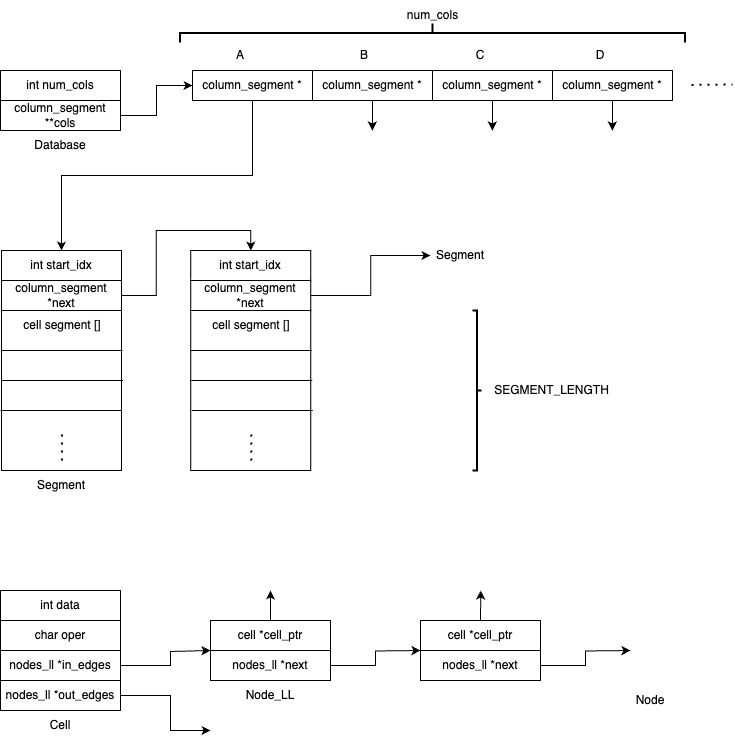
\includegraphics[width=0.5\textwidth]{docs/hld.png}
    \caption{High-Level Design of the Database}
    \label{fig:high_level_design}
\end{figure}

\section{Data Structures Used}
To ensure efficient performance, the following data structures were utilized:
\begin{itemize}
    \item \textbf{Linked List}: Used to manage edges in the dependency graph.
    \item \textbf{Graph (Dependency Graph)}: Tracks dependencies between cells for formula calculations.
    \item \textbf{Deque}: Implements efficient column-wise storage of cell data.
\end{itemize}

\section{Features and Implementation}
\subsection{Storage}
The smallest storage unit is cell, which stores int data, a character oper indicating the type of operation that is performed on the cell(e.g. A1=3 then oper=1, A1=A2-A3 then oper=4), two linked lists of cell pointers for storing dependencies, one for in-dependency and other for out-dependency. Cells in out-dependency linked list are dependent on the cell, while cells in in-dependency influence the cell. For example, in the relation A1=A2+A3, A2 and A3 will be in in-dependency of A1 while A1 will be in out-dependency of A2 and A3.\\
Above that, we have a deque like structure: column segment. Each segment stores the cells of a column of a particular range to ensure that only those segments are malloc'd that we need. Each segment has a starting index, they store cells from that index till index + SEGMENT-LENGTH. Whenever data has to be added, all the linked segments are traversed and their start-idx are checked. If the segment for the row has not been initialized, then we initialize a new segment and append it to the end of the segment chain.\\
Sample insertion sequence for a column:
\begin{verbatim}
set(row=123, data=10): [start_idx = 100 | 0, ..., 10, 0, ...] -> NULL
set(row=999, data=1):  [start_idx = 100 | 0, ..., 10, 0, ...] -> 
                        [start_idx = 900 | 0, ..., 1] -> NULL
set(row=0, data=99):   [start_idx = 100 | 0, ..., 10, 0, ...] -> 
                        [start_idx = 900 | 0, ..., 1] -> [start_idx = 0 | 99, 0, ...] -> NULL
\end{verbatim}
All the interaction of the code with the data stored is through the database struct, which simply contains an array of pointers to individual column segments. Initially, all pointers are NULL, and they are malloc'd as and when needed. Functions are implemented to allow getting and setting data among other functions.

\subsection{Handling dependencies}
The application uses a directed graph to represent cell dependencies. Each cell struct stores dependencies in two linked lists: in\_edges (cells this cell depends on) and out\_edges (cells that depend on this cell). When a cell's formula references others, these references are recorded as dependencies. To ensure that there are no loops, cycle detection is performed, preventing circular references. Evaluation order is determined via topological sorting, guaranteeing that dependent cells are updated before their referencing cells. Error propagation ensures that if a cell contains an error, all cells depending on it also reflect that error, maintaining spreadsheet consistency.

\subsection{Parser and Evaluator}
User commands are processed through a two-stage pipeline: parsing and evaluation. The parser function analyzes input strings, validating syntax and extracting command details into a response struct. This struct encapsulates the operation, target cell, arguments, and any parsing errors. The evaluator then receives this struct, handling dependency management, cell evaluation, and database updates. It constructs and manages a dependency graph, detects cycles, and performs topological sorting to ensure correct evaluation order. The evaluator also propagates errors and controls the display state and top-left cell.\\
During evaluation, cells are updated based on their formulas, which can include arithmetic operations, function calls, or direct assignments. The evaluator ensures data consistency by propagating errors from dependent cells and preventing circular dependencies. It utilizes helper functions to compute connected components and manage isolated cells for constant values. The resulting changes are reflected in the spreadsheet's database, which the display component then renders to the user.

\subsection{Cycle detection}
Whenever a new relation is added in the sheet, we check if cycle is formed on adding the new dependencies. First we store the state of the cell being modified. Then we remove the old dependencies and add new links. We check for cycles, and if there is a cycle, we restore the state of the cell.\\
To check for cycles, we traverse the dependency graph depth-first. While traversing the graph, if we encounter a cell that is in the current branch of dfs tree, we know that there is a cycle.


\section{Integration and Workflow}
When a user inputs a command, the following steps occur:
\begin{enumerate}
    \item The input is passed to the parser, which categorizes it and returns a response.
    \item If it is a formula, dependencies are analyzed using a graph structure.
    \item The evaluator computes the value if necessary and updates the data storage.
    \item The UI updates the display to reflect changes.
\end{enumerate}


\section{Challenges and Future Scope}
Some of the challenges encountered include:
\begin{itemize}
    \item Efficiently handling formula dependencies and cyclic references.
    \item Managing memory usage for large spreadsheets.
    \item Optimizing the number of mallocs, and hence frees.
\end{itemize}
Some features we can implement at a later stage include:
\begin{itemize}
    \item Malloc pooling to prevent frequent mallocs and frees which are bottlenecks in the current implementation.
    \item Implementing lazy evaluation for improved performance.
\end{itemize}

\section{Submission Links}
Link to GitHub: \url{https://github.com/mantros2003/cop290_spreadsheet}\\
Link to demo video: \url{https://csciitd-my.sharepoint.com/:v:/g/personal/me2221540_iitd_ac_in/EYr-Abg-zm5CtpkQ88GJsSgBnPjcnUUmsg4KP-BE_Kez5g?nav=eyJyZWZlcnJhbEluZm8iOnsicmVmZXJyYWxBcHAiOiJPbmVEcml2ZUZvckJ1c2luZXNzIiwicmVmZXJyYWxBcHBQbGF0Zm9ybSI6IldlYiIsInJlZmVycmFsTW9kZSI6InZpZXciLCJyZWZlcnJhbFZpZXciOiJNeUZpbGVzTGlua0NvcHkifX0&e=7S4x7s}

\section{Conclusion}
This project successfully implements a functional spreadsheet application for terminal users. With its modular architecture, efficient data handling, and core spreadsheet functionalities, it provides a lightweight alternative to traditional GUI-based spreadsheets. Future enhancements may include advanced functions, improved UI, and multi-user collaboration features.

\end{document}
